% Options for packages loaded elsewhere
\PassOptionsToPackage{unicode}{hyperref}
\PassOptionsToPackage{hyphens}{url}
%
\documentclass[
]{article}
\usepackage{amsmath,amssymb}
\usepackage{lmodern}
\usepackage{iftex}
\ifPDFTeX
  \usepackage[T1]{fontenc}
  \usepackage[utf8]{inputenc}
  \usepackage{textcomp} % provide euro and other symbols
\else % if luatex or xetex
  \usepackage{unicode-math}
  \defaultfontfeatures{Scale=MatchLowercase}
  \defaultfontfeatures[\rmfamily]{Ligatures=TeX,Scale=1}
\fi
% Use upquote if available, for straight quotes in verbatim environments
\IfFileExists{upquote.sty}{\usepackage{upquote}}{}
\IfFileExists{microtype.sty}{% use microtype if available
  \usepackage[]{microtype}
  \UseMicrotypeSet[protrusion]{basicmath} % disable protrusion for tt fonts
}{}
\makeatletter
\@ifundefined{KOMAClassName}{% if non-KOMA class
  \IfFileExists{parskip.sty}{%
    \usepackage{parskip}
  }{% else
    \setlength{\parindent}{0pt}
    \setlength{\parskip}{6pt plus 2pt minus 1pt}}
}{% if KOMA class
  \KOMAoptions{parskip=half}}
\makeatother
\usepackage{xcolor}
\usepackage[margin=1in]{geometry}
\usepackage{color}
\usepackage{fancyvrb}
\newcommand{\VerbBar}{|}
\newcommand{\VERB}{\Verb[commandchars=\\\{\}]}
\DefineVerbatimEnvironment{Highlighting}{Verbatim}{commandchars=\\\{\}}
% Add ',fontsize=\small' for more characters per line
\usepackage{framed}
\definecolor{shadecolor}{RGB}{248,248,248}
\newenvironment{Shaded}{\begin{snugshade}}{\end{snugshade}}
\newcommand{\AlertTok}[1]{\textcolor[rgb]{0.94,0.16,0.16}{#1}}
\newcommand{\AnnotationTok}[1]{\textcolor[rgb]{0.56,0.35,0.01}{\textbf{\textit{#1}}}}
\newcommand{\AttributeTok}[1]{\textcolor[rgb]{0.77,0.63,0.00}{#1}}
\newcommand{\BaseNTok}[1]{\textcolor[rgb]{0.00,0.00,0.81}{#1}}
\newcommand{\BuiltInTok}[1]{#1}
\newcommand{\CharTok}[1]{\textcolor[rgb]{0.31,0.60,0.02}{#1}}
\newcommand{\CommentTok}[1]{\textcolor[rgb]{0.56,0.35,0.01}{\textit{#1}}}
\newcommand{\CommentVarTok}[1]{\textcolor[rgb]{0.56,0.35,0.01}{\textbf{\textit{#1}}}}
\newcommand{\ConstantTok}[1]{\textcolor[rgb]{0.00,0.00,0.00}{#1}}
\newcommand{\ControlFlowTok}[1]{\textcolor[rgb]{0.13,0.29,0.53}{\textbf{#1}}}
\newcommand{\DataTypeTok}[1]{\textcolor[rgb]{0.13,0.29,0.53}{#1}}
\newcommand{\DecValTok}[1]{\textcolor[rgb]{0.00,0.00,0.81}{#1}}
\newcommand{\DocumentationTok}[1]{\textcolor[rgb]{0.56,0.35,0.01}{\textbf{\textit{#1}}}}
\newcommand{\ErrorTok}[1]{\textcolor[rgb]{0.64,0.00,0.00}{\textbf{#1}}}
\newcommand{\ExtensionTok}[1]{#1}
\newcommand{\FloatTok}[1]{\textcolor[rgb]{0.00,0.00,0.81}{#1}}
\newcommand{\FunctionTok}[1]{\textcolor[rgb]{0.00,0.00,0.00}{#1}}
\newcommand{\ImportTok}[1]{#1}
\newcommand{\InformationTok}[1]{\textcolor[rgb]{0.56,0.35,0.01}{\textbf{\textit{#1}}}}
\newcommand{\KeywordTok}[1]{\textcolor[rgb]{0.13,0.29,0.53}{\textbf{#1}}}
\newcommand{\NormalTok}[1]{#1}
\newcommand{\OperatorTok}[1]{\textcolor[rgb]{0.81,0.36,0.00}{\textbf{#1}}}
\newcommand{\OtherTok}[1]{\textcolor[rgb]{0.56,0.35,0.01}{#1}}
\newcommand{\PreprocessorTok}[1]{\textcolor[rgb]{0.56,0.35,0.01}{\textit{#1}}}
\newcommand{\RegionMarkerTok}[1]{#1}
\newcommand{\SpecialCharTok}[1]{\textcolor[rgb]{0.00,0.00,0.00}{#1}}
\newcommand{\SpecialStringTok}[1]{\textcolor[rgb]{0.31,0.60,0.02}{#1}}
\newcommand{\StringTok}[1]{\textcolor[rgb]{0.31,0.60,0.02}{#1}}
\newcommand{\VariableTok}[1]{\textcolor[rgb]{0.00,0.00,0.00}{#1}}
\newcommand{\VerbatimStringTok}[1]{\textcolor[rgb]{0.31,0.60,0.02}{#1}}
\newcommand{\WarningTok}[1]{\textcolor[rgb]{0.56,0.35,0.01}{\textbf{\textit{#1}}}}
\usepackage{graphicx}
\makeatletter
\def\maxwidth{\ifdim\Gin@nat@width>\linewidth\linewidth\else\Gin@nat@width\fi}
\def\maxheight{\ifdim\Gin@nat@height>\textheight\textheight\else\Gin@nat@height\fi}
\makeatother
% Scale images if necessary, so that they will not overflow the page
% margins by default, and it is still possible to overwrite the defaults
% using explicit options in \includegraphics[width, height, ...]{}
\setkeys{Gin}{width=\maxwidth,height=\maxheight,keepaspectratio}
% Set default figure placement to htbp
\makeatletter
\def\fps@figure{htbp}
\makeatother
\setlength{\emergencystretch}{3em} % prevent overfull lines
\providecommand{\tightlist}{%
  \setlength{\itemsep}{0pt}\setlength{\parskip}{0pt}}
\setcounter{secnumdepth}{-\maxdimen} % remove section numbering
\ifLuaTeX
  \usepackage{selnolig}  % disable illegal ligatures
\fi
\IfFileExists{bookmark.sty}{\usepackage{bookmark}}{\usepackage{hyperref}}
\IfFileExists{xurl.sty}{\usepackage{xurl}}{} % add URL line breaks if available
\urlstyle{same} % disable monospaced font for URLs
\hypersetup{
  pdftitle={EDA song sparrow data},
  hidelinks,
  pdfcreator={LaTeX via pandoc}}

\title{EDA song sparrow data}
\author{}
\date{\vspace{-2.5em}2023-01-17}

\begin{document}
\maketitle

\hypertarget{data-frame-overview}{%
\subsection*{Data frame overview}\label{data-frame-overview}}
\addcontentsline{toc}{subsection}{Data frame overview}

\hypertarget{pedigree}{%
\subsubsection*{Pedigree}\label{pedigree}}
\addcontentsline{toc}{subsubsection}{Pedigree}

The first object is \texttt{d.ped} which contains the pedigree
information.

\begin{Shaded}
\begin{Highlighting}[]
\FunctionTok{summary}\NormalTok{(d.ped)}
\end{Highlighting}
\end{Shaded}

\begin{verbatim}
##     ninecode             gendam             gensire         
##  Min.   :109137448   Min.   :109137468   Min.   :109137448  
##  1st Qu.:146164012   1st Qu.:146130794   1st Qu.:146130313  
##  Median :176124850   Median :176124382   Median :176124004  
##  Mean   :196520240   Mean   :188116000   Mean   :185463038  
##  3rd Qu.:243185045   3rd Qu.:226189260   3rd Qu.:226189228  
##  Max.   :999999999   Max.   :999999999   Max.   :266176829  
##                      NA's   :59          NA's   :59
\end{verbatim}

It has the columns \emph{ninecode}, \emph{gendam}, and \emph{gensire}.
The first column cannot be \texttt{NA} and is the unique identifier for
an individual, whereas \texttt{gendam}and \texttt{gensire} are
references (foreign keys) to the known maternal and paternal link,
respectively. Both of these columns have 59 NAs. In fact, these NAs
overlap completely since they are the founder population with no defined
paternal or maternal link:

\begin{Shaded}
\begin{Highlighting}[]
\NormalTok{d.ped[}\FunctionTok{is.na}\NormalTok{(d.ped}\SpecialCharTok{$}\NormalTok{gendam), }\StringTok{"gensire"}\NormalTok{]}
\end{Highlighting}
\end{Shaded}

\begin{verbatim}
##  [1] NA NA NA NA NA NA NA NA NA NA NA NA NA NA NA NA NA NA NA NA NA NA NA NA NA
## [26] NA NA NA NA NA NA NA NA NA NA NA NA NA NA NA NA NA NA NA NA NA NA NA NA NA
## [51] NA NA NA NA NA NA NA NA NA
\end{verbatim}

We see that \emph{gensire} is NA for all instances where \emph{gendam}
is also NA. This is in fact the founder population with no defined
parental linkage.

\hypertarget{d.q}{%
\subsubsection*{d.Q}\label{d.q}}
\addcontentsline{toc}{subsubsection}{d.Q}

This table has the columns \emph{g1}, \emph{foc0} and \emph{ninecode}
(ID).

\begin{Shaded}
\begin{Highlighting}[]
\FunctionTok{head}\NormalTok{(d.Q)}
\end{Highlighting}
\end{Shaded}

\begin{verbatim}
##   foc0 g1  ninecode
## 1    1  0 109137407
## 2    1  0 109137408
## 3    1  0 109137418
## 4    1  0 109137420
## 5    1  0 109137421
## 6    1  0 109137425
\end{verbatim}

From the first look, it might seem like these are binary/categorical
variables, but plotting the values across indices show that the order of
the rows are structured so that they start at 1 and 0 respectively.

\begin{Shaded}
\begin{Highlighting}[]
\FunctionTok{par}\NormalTok{(}\AttributeTok{mfrow =} \FunctionTok{c}\NormalTok{(}\DecValTok{1}\NormalTok{, }\DecValTok{2}\NormalTok{))}
\FunctionTok{plot}\NormalTok{(d.Q}\SpecialCharTok{$}\NormalTok{g1, }\AttributeTok{main =} \StringTok{"g1"}\NormalTok{)}
\FunctionTok{plot}\NormalTok{(d.Q}\SpecialCharTok{$}\NormalTok{foc0, }\AttributeTok{main =} \StringTok{"foc0"}\NormalTok{)}
\end{Highlighting}
\end{Shaded}

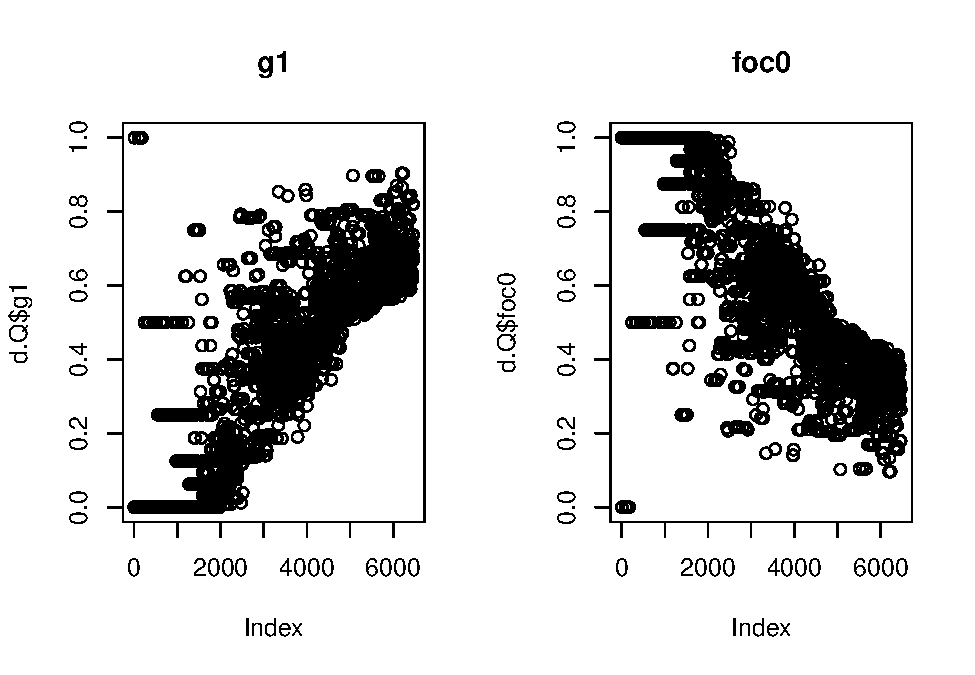
\includegraphics{EDA_files/figure-latex/unnamed-chunk-2-1.pdf}

We can also look at the correlation between these two values

\begin{Shaded}
\begin{Highlighting}[]
\FunctionTok{cor}\NormalTok{(d.Q}\SpecialCharTok{$}\NormalTok{foc0, d.Q}\SpecialCharTok{$}\NormalTok{g1)}
\end{Highlighting}
\end{Shaded}

\begin{verbatim}
## [1] -1
\end{verbatim}

We have a very strong negative correlation here. We can also look at the
individuals whose ID were in the \emph{founder population}:

\begin{Shaded}
\begin{Highlighting}[]
\NormalTok{founder\_population.id }\OtherTok{\textless{}{-}}\NormalTok{ d.ped[}\FunctionTok{is.na}\NormalTok{(d.ped}\SpecialCharTok{$}\NormalTok{gendam), }\StringTok{"ninecode"}\NormalTok{]}
\FunctionTok{table}\NormalTok{(d.Q[}\FunctionTok{which}\NormalTok{(d.Q}\SpecialCharTok{$}\NormalTok{ninecode }\SpecialCharTok{\%in\%}\NormalTok{ founder\_population.id), }\FunctionTok{c}\NormalTok{(}\StringTok{"foc0"}\NormalTok{, }\StringTok{"g1"}\NormalTok{)])}
\end{Highlighting}
\end{Shaded}

\begin{verbatim}
##     g1
## foc0  0  1
##    0  0 33
##    1 26  0
\end{verbatim}

The values seem to be relatively balanced between \(0\) and \(1\) in the
founder population. This supports the idea that they measure the
immigration contribution to the genetic composition of the individuals.
All immigrant individuals are completely immigrant, have no pedigree and
are thus part of the founder population. The latter are those who are
the ``inital'' natives on the island, meaning that their values must be
exactly zero.

\hypertarget{ped.prune}{%
\subsubsection*{ped.prune}\label{ped.prune}}
\addcontentsline{toc}{subsubsection}{ped.prune}

This is a pruned pedigree, only considering the 1993-2018 observations
but also combining the knowledge of the 1975-1992 observations into
them.

\hypertarget{qg.data.gg.ind}{%
\subsubsection*{qg.data.gg.ind}\label{qg.data.gg.ind}}
\addcontentsline{toc}{subsubsection}{qg.data.gg.ind}

This object has the following shape:

\begin{Shaded}
\begin{Highlighting}[]
\FunctionTok{head}\NormalTok{(qg.data.gg.inds)}
\end{Highlighting}
\end{Shaded}

\begin{verbatim}
##    ninecode natalyr sex.use nestrec surv.ind.to.ad brood.date sex.use.x1
## 1 111111112    2012       0    3086              0        120          1
## 2 111111121    2015       0    3237              0        141          1
## 3 143173366    1993       1    1838              1         96          1
## 4 143173381    1993       2    1867              1        102          2
## 5 143173382    1993       1    1867              0        102          1
## 6 143173384    1993       1    1851              0        102          1
##       f.coef      foc0        g1 natalyr.no sex
## 1 0.11155218 0.4085679 0.5914321         38   0
## 2 0.04814660 0.3299752 0.6700248         41   0
## 3 0.05108643 0.5283203 0.4716797         19   0
## 4 0.03125000 0.6250000 0.3750000         19   1
## 5 0.03417969 0.4335938 0.5664062         19   0
## 6 0.02148438 0.6328125 0.3671875         19   0
\end{verbatim}

The response variable we will use is \texttt{surv.ind.to.ad}. Some
immediate observations:

\begin{Shaded}
\begin{Highlighting}[]
\FunctionTok{paste}\NormalTok{(}\StringTok{"Earliest year:"}\NormalTok{, }\FunctionTok{min}\NormalTok{(qg.data.gg.inds}\SpecialCharTok{$}\NormalTok{natalyr))}
\end{Highlighting}
\end{Shaded}

\begin{verbatim}
## [1] "Earliest year: 1993"
\end{verbatim}

\begin{Shaded}
\begin{Highlighting}[]
\FunctionTok{paste}\NormalTok{(}\FunctionTok{c}\NormalTok{(}\StringTok{"Number not survived:"}\NormalTok{, }\StringTok{"Number survived:"}\NormalTok{), }\FunctionTok{table}\NormalTok{(qg.data.gg.inds}\SpecialCharTok{$}\NormalTok{surv.ind.to.ad))}
\end{Highlighting}
\end{Shaded}

\begin{verbatim}
## [1] "Number not survived: 1817" "Number survived: 661"
\end{verbatim}

\begin{Shaded}
\begin{Highlighting}[]
\FunctionTok{paste}\NormalTok{(}\StringTok{"natal year correlation:"}\NormalTok{, }\FunctionTok{cor}\NormalTok{(qg.data.gg.inds}\SpecialCharTok{$}\NormalTok{natalyr, qg.data.gg.inds}\SpecialCharTok{$}\NormalTok{natalyr.no))}
\end{Highlighting}
\end{Shaded}

\begin{verbatim}
## [1] "natal year correlation: 1"
\end{verbatim}

\begin{Shaded}
\begin{Highlighting}[]
\FunctionTok{paste}\NormalTok{(}\StringTok{"correlation between sex and sex.x1:"}\NormalTok{, }\FunctionTok{cor}\NormalTok{(qg.data.gg.inds}\SpecialCharTok{$}\NormalTok{sex.use, qg.data.gg.inds}\SpecialCharTok{$}\NormalTok{sex.use.x1))}
\end{Highlighting}
\end{Shaded}

\begin{verbatim}
## [1] "correlation between sex and sex.x1: 0.842997540673555"
\end{verbatim}

An overview over the columns:

\begin{itemize}
\tightlist
\item
  \emph{ninecode}: Individual ID
\item
  \emph{natalyr}: Year individual was born, e.g.~2015.
\item
  \emph{sex.use}: \textbf{Not in use}
\item
  \emph{nestrec}: ID for nest number
\item
  \emph{brood.date}: Day of the year when the first offspring in
  individuals nest hatched (I think zero is April 1st, it's in Rekkebo
  thesis)
\item
  \emph{sex.use.x1}: Sex of individual, 1 or 2
\item
  \emph{f.coef}: Inbreeding coefficient
\item
  \emph{foc0}: ``How foreign'' individual is, related to f.coef
\item
  \emph{g1}: Inverse of \emph{foc0} essentially.
\item
  \emph{natalyr.no}: The same as natal year, starting with 1974 as 0
  (2015=41).
\end{itemize}

\hypertarget{vizualization-of-juvenile-survival}{%
\subsection*{Vizualization of juvenile
survival}\label{vizualization-of-juvenile-survival}}
\addcontentsline{toc}{subsection}{Vizualization of juvenile survival}

We will have a look at how the response, juveniule survival, realtes to
the other covariates in our data.

First, we look at sex:

\begin{Shaded}
\begin{Highlighting}[]
\FunctionTok{library}\NormalTok{(ggplot2)}
\end{Highlighting}
\end{Shaded}

\begin{verbatim}
## Warning: package 'ggplot2' was built under R version 4.2.2
\end{verbatim}

\begin{Shaded}
\begin{Highlighting}[]
\FunctionTok{ggplot}\NormalTok{(qg.data.gg.inds, }\FunctionTok{aes}\NormalTok{(}\AttributeTok{x =} \FunctionTok{factor}\NormalTok{(surv.ind.to.ad), }\AttributeTok{fill =} \FunctionTok{factor}\NormalTok{(sex))) }\SpecialCharTok{+}
  \FunctionTok{ggtitle}\NormalTok{(}\StringTok{"Distribution of juvenile survival to adulthood"}\NormalTok{) }\SpecialCharTok{+}
  \FunctionTok{geom\_bar}\NormalTok{(}\AttributeTok{alpha =} \FloatTok{0.7}\NormalTok{) }\SpecialCharTok{+}
  \FunctionTok{xlab}\NormalTok{(}\StringTok{"Survival"}\NormalTok{) }\SpecialCharTok{+}
  \FunctionTok{scale\_fill\_manual}\NormalTok{(}
    \AttributeTok{name =} \StringTok{"Sex"}\NormalTok{,}
    \AttributeTok{labels =} \FunctionTok{c}\NormalTok{(}\StringTok{"Male"}\NormalTok{, }\StringTok{"Female"}\NormalTok{),}
    \AttributeTok{values =} \FunctionTok{c}\NormalTok{(}\StringTok{"\#619CFF"}\NormalTok{, }\StringTok{"\#F8766D"}\NormalTok{)}
\NormalTok{  )}
\end{Highlighting}
\end{Shaded}

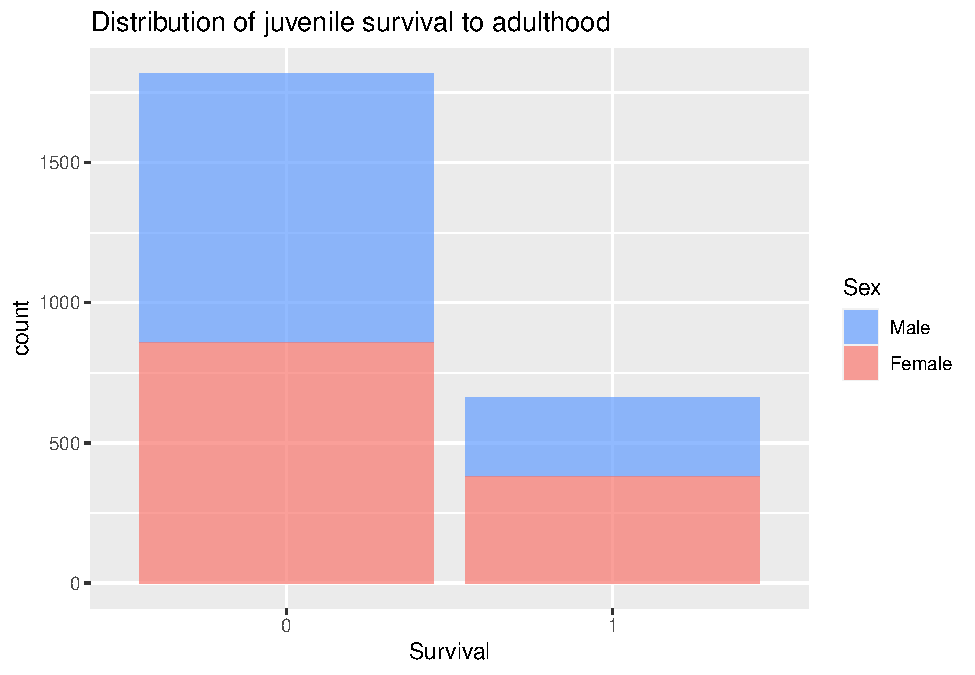
\includegraphics{EDA_files/figure-latex/unnamed-chunk-7-1.pdf}

Seems like the sex in relation to survival is relatively balanced here.
We can note that it seems like a larger portion of those surviving are
females. Next, we look at the breeding coefficient.

\begin{Shaded}
\begin{Highlighting}[]
\FunctionTok{ggplot}\NormalTok{(qg.data.gg.inds, }\FunctionTok{aes}\NormalTok{(}\AttributeTok{x =}\NormalTok{ f.coef, }\AttributeTok{fill =} \FunctionTok{factor}\NormalTok{(surv.ind.to.ad))) }\SpecialCharTok{+}
  \FunctionTok{ggtitle}\NormalTok{(}\StringTok{"Distribution of inbreeding coefficient"}\NormalTok{) }\SpecialCharTok{+}
  \FunctionTok{geom\_density}\NormalTok{(}\AttributeTok{alpha =} \FloatTok{0.5}\NormalTok{) }\SpecialCharTok{+}
  \FunctionTok{xlab}\NormalTok{(}\StringTok{"Inbreeding coefficient"}\NormalTok{) }\SpecialCharTok{+}
  \FunctionTok{ylab}\NormalTok{(}\StringTok{"Density"}\NormalTok{) }\SpecialCharTok{+}
  \FunctionTok{scale\_fill\_manual}\NormalTok{(}
    \AttributeTok{name =} \StringTok{"Survived to adulthood"}\NormalTok{,}
    \AttributeTok{label =} \FunctionTok{c}\NormalTok{(}\StringTok{"No"}\NormalTok{, }\StringTok{"Yes"}\NormalTok{),}
    \AttributeTok{values =} \FunctionTok{c}\NormalTok{(}\StringTok{"\#D55E00"}\NormalTok{, }\StringTok{"\#009E73"}\NormalTok{)}
\NormalTok{  )}
\end{Highlighting}
\end{Shaded}

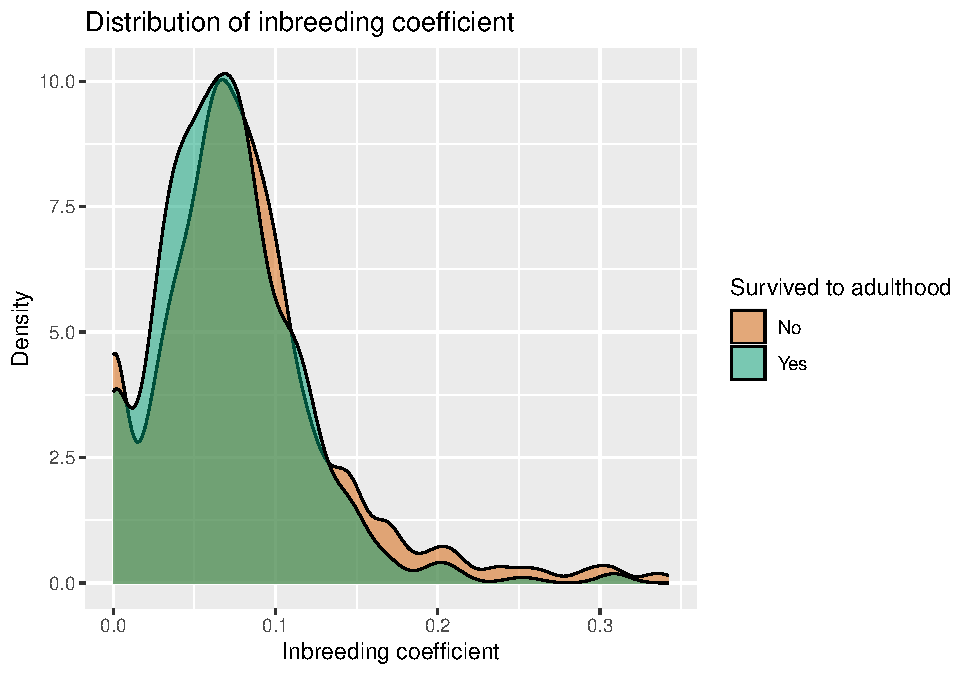
\includegraphics{EDA_files/figure-latex/unnamed-chunk-8-1.pdf}

Here we see that survival is a bit more skewed towards lower inbreeding
coefficients. We can also look at how the proportion of individuals have
survived over the years:

\begin{Shaded}
\begin{Highlighting}[]
\FunctionTok{ggplot}\NormalTok{(}\FunctionTok{aggregate}\NormalTok{(surv.ind.to.ad }\SpecialCharTok{\textasciitilde{}}\NormalTok{ natalyr, qg.data.gg.inds, }\ControlFlowTok{function}\NormalTok{(x) \{}
  \FunctionTok{sum}\NormalTok{(x) }\SpecialCharTok{/} \FunctionTok{length}\NormalTok{(x)}
\NormalTok{\}), }\FunctionTok{aes}\NormalTok{(}\AttributeTok{x =}\NormalTok{ natalyr, }\AttributeTok{y =}\NormalTok{ surv.ind.to.ad)) }\SpecialCharTok{+}
  \FunctionTok{geom\_line}\NormalTok{() }\SpecialCharTok{+}
  \FunctionTok{geom\_point}\NormalTok{() }\SpecialCharTok{+}
  \FunctionTok{geom\_smooth}\NormalTok{() }\SpecialCharTok{+}
  \FunctionTok{ggtitle}\NormalTok{(}\StringTok{"Portion of juvenile survival by year"}\NormalTok{) }\SpecialCharTok{+}
  \FunctionTok{xlab}\NormalTok{(}\StringTok{"Year"}\NormalTok{) }\SpecialCharTok{+}
  \FunctionTok{ylab}\NormalTok{(}\StringTok{"Portion survived"}\NormalTok{) }\SpecialCharTok{+}
  \FunctionTok{scale\_x\_continuous}\NormalTok{(}\AttributeTok{breaks =} \FunctionTok{seq}\NormalTok{(}\DecValTok{1993}\NormalTok{, }\DecValTok{2018}\NormalTok{, }\AttributeTok{by =} \DecValTok{4}\NormalTok{))}
\end{Highlighting}
\end{Shaded}

\begin{verbatim}
## `geom_smooth()` using method = 'loess' and formula = 'y ~ x'
\end{verbatim}

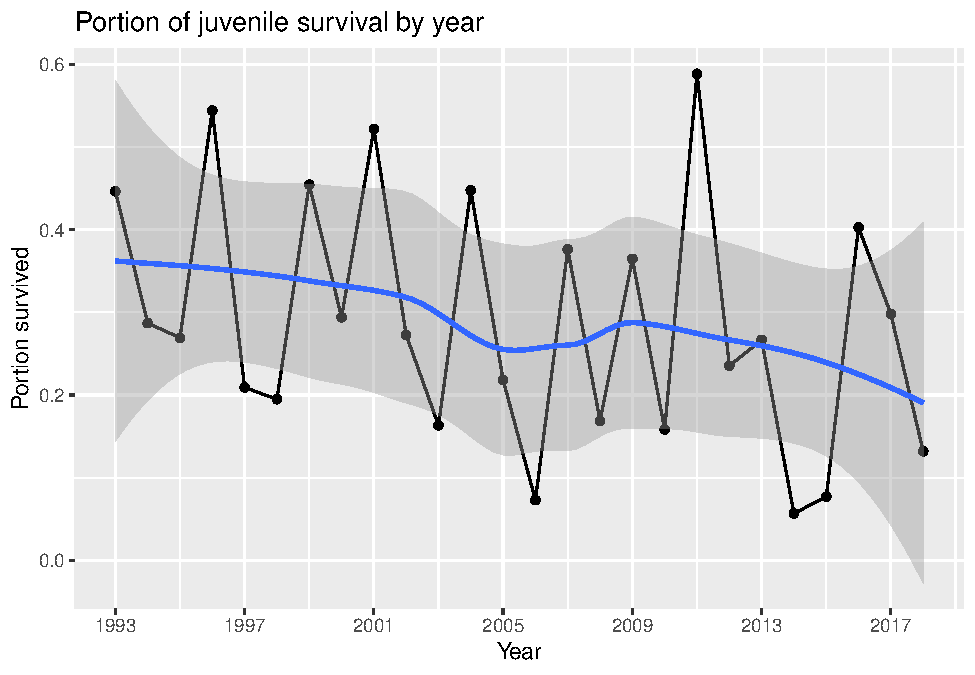
\includegraphics{EDA_files/figure-latex/unnamed-chunk-9-1.pdf}

There seem to be very little trending along the years, but possibly a
small negative trend. Let's also see if there is some correspondence
between genetic group coefficient (\texttt{g1}) and juvenile survival.

\begin{Shaded}
\begin{Highlighting}[]
\FunctionTok{ggplot}\NormalTok{(qg.data.gg.inds, }\FunctionTok{aes}\NormalTok{(}\AttributeTok{x =}\NormalTok{ g1, }\AttributeTok{fill =} \FunctionTok{factor}\NormalTok{(surv.ind.to.ad))) }\SpecialCharTok{+}
  \FunctionTok{ggtitle}\NormalTok{(}\StringTok{"Distribution of genetic group coefficient"}\NormalTok{) }\SpecialCharTok{+}
  \FunctionTok{geom\_density}\NormalTok{(}\AttributeTok{alpha =} \FloatTok{0.5}\NormalTok{) }\SpecialCharTok{+}
  \FunctionTok{xlab}\NormalTok{(}\StringTok{"Genetic group coefficient"}\NormalTok{) }\SpecialCharTok{+}
  \FunctionTok{ylab}\NormalTok{(}\StringTok{"Density"}\NormalTok{) }\SpecialCharTok{+}
  \FunctionTok{scale\_fill\_manual}\NormalTok{(}
    \AttributeTok{name =} \StringTok{"Survived to adulthood"}\NormalTok{,}
    \AttributeTok{label =} \FunctionTok{c}\NormalTok{(}\StringTok{"No"}\NormalTok{, }\StringTok{"Yes"}\NormalTok{),}
    \AttributeTok{values =} \FunctionTok{c}\NormalTok{(}\StringTok{"\#D55E00"}\NormalTok{, }\StringTok{"\#009E73"}\NormalTok{)}
\NormalTok{  )}
\end{Highlighting}
\end{Shaded}

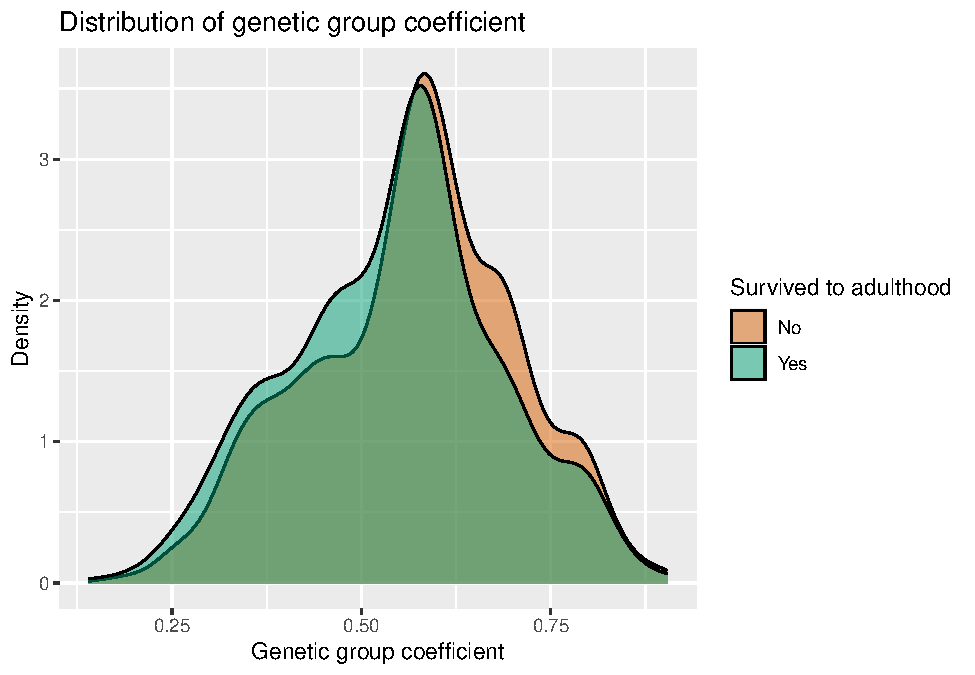
\includegraphics{EDA_files/figure-latex/unnamed-chunk-10-1.pdf}

This shows a similar result to the inbreeding coefficient, namely a skew
towards the right (lower values of coefficient) in the group that
survived. We might also look into survival based on brood date:

\begin{Shaded}
\begin{Highlighting}[]
\FunctionTok{ggplot}\NormalTok{(}\FunctionTok{aggregate}\NormalTok{(surv.ind.to.ad }\SpecialCharTok{\textasciitilde{}}\NormalTok{ brood.date, qg.data.gg.inds, }\ControlFlowTok{function}\NormalTok{(x) \{}
  \FunctionTok{sum}\NormalTok{(x) }\SpecialCharTok{/} \FunctionTok{length}\NormalTok{(x)}
\NormalTok{\}), }\FunctionTok{aes}\NormalTok{(}\AttributeTok{x =}\NormalTok{ brood.date, }\AttributeTok{y =}\NormalTok{ surv.ind.to.ad)) }\SpecialCharTok{+}
  \FunctionTok{geom\_line}\NormalTok{() }\SpecialCharTok{+}
  \FunctionTok{geom\_point}\NormalTok{() }\SpecialCharTok{+}
  \FunctionTok{geom\_smooth}\NormalTok{() }\SpecialCharTok{+}
  \FunctionTok{ggtitle}\NormalTok{(}\StringTok{"Portion of juvenile survival by brood date"}\NormalTok{) }\SpecialCharTok{+}
  \FunctionTok{xlab}\NormalTok{(}\StringTok{"Brood date"}\NormalTok{) }\SpecialCharTok{+}
  \FunctionTok{ylab}\NormalTok{(}\StringTok{"Portion survived"}\NormalTok{)}
\end{Highlighting}
\end{Shaded}

\begin{verbatim}
## `geom_smooth()` using method = 'loess' and formula = 'y ~ x'
\end{verbatim}

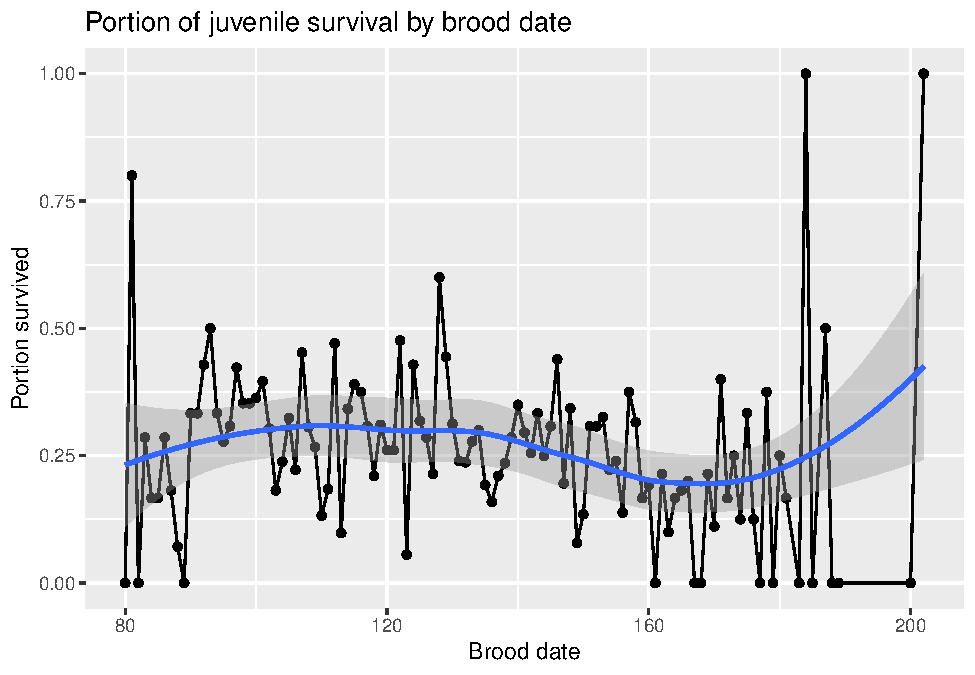
\includegraphics{EDA_files/figure-latex/unnamed-chunk-11-1.pdf}

This last plot seem to indicate that survival is relatively stable and
somewhat decreasing for those hatched relatively late. For the largest
values of brood date, we get an increasing trend but also much
uncertainty since not that many were hatched this late.

\end{document}
